\section{Introdução} \label{section: Introducao}
\setstretch{1.15}
Nos dias de hoje, a escolha entre sistemas operativos open source e proprietários é uma decisão crucial para empresas. Esta escolha envolve uma série de considerações, desde o núcleo (kernel) do sistema até às implicações legais do licenciamento e às preocupações com a segurança e estabilidade.
\par \vspace{6pt}
Neste trabalho iremos explorar estes tópicos fazendo a comparação entre sistemas operativos \textit{open source} e proprietários apresentando as suas características.
Destacamos também a importância do \textit{kernel} e as suas responsabilidades na operação do sistema operativo.
\par \vspace{6pt}
Analisando o caso específico do Linux, falamos um pouco da sua historia e importância do kernel Linux e do projecto GNU e exemplificamos diferentes utilizações actuais deste sistema.
\par \vspace{6pt}
Discutimos as complexidades do licenciamento open source, examinando as implicações legais e práticas para empresas que optem por utilizar software de \textit{open source}.
\par \vspace{6pt}
Ao longo deste trabalho, também investigaremos a segurança dos sistemas operativos open source, analizando quais os principais riscos no seu uso. Por fim, analisaremos o processo de utilização de software open source em ambientes empresariais, explorando os desafios e benefícios associados à adoção deste modelo de software.
\vspace{12pt}
\begin{figure}[H]
  \centering
  % width=\textwidth para imagem da largura do texto
  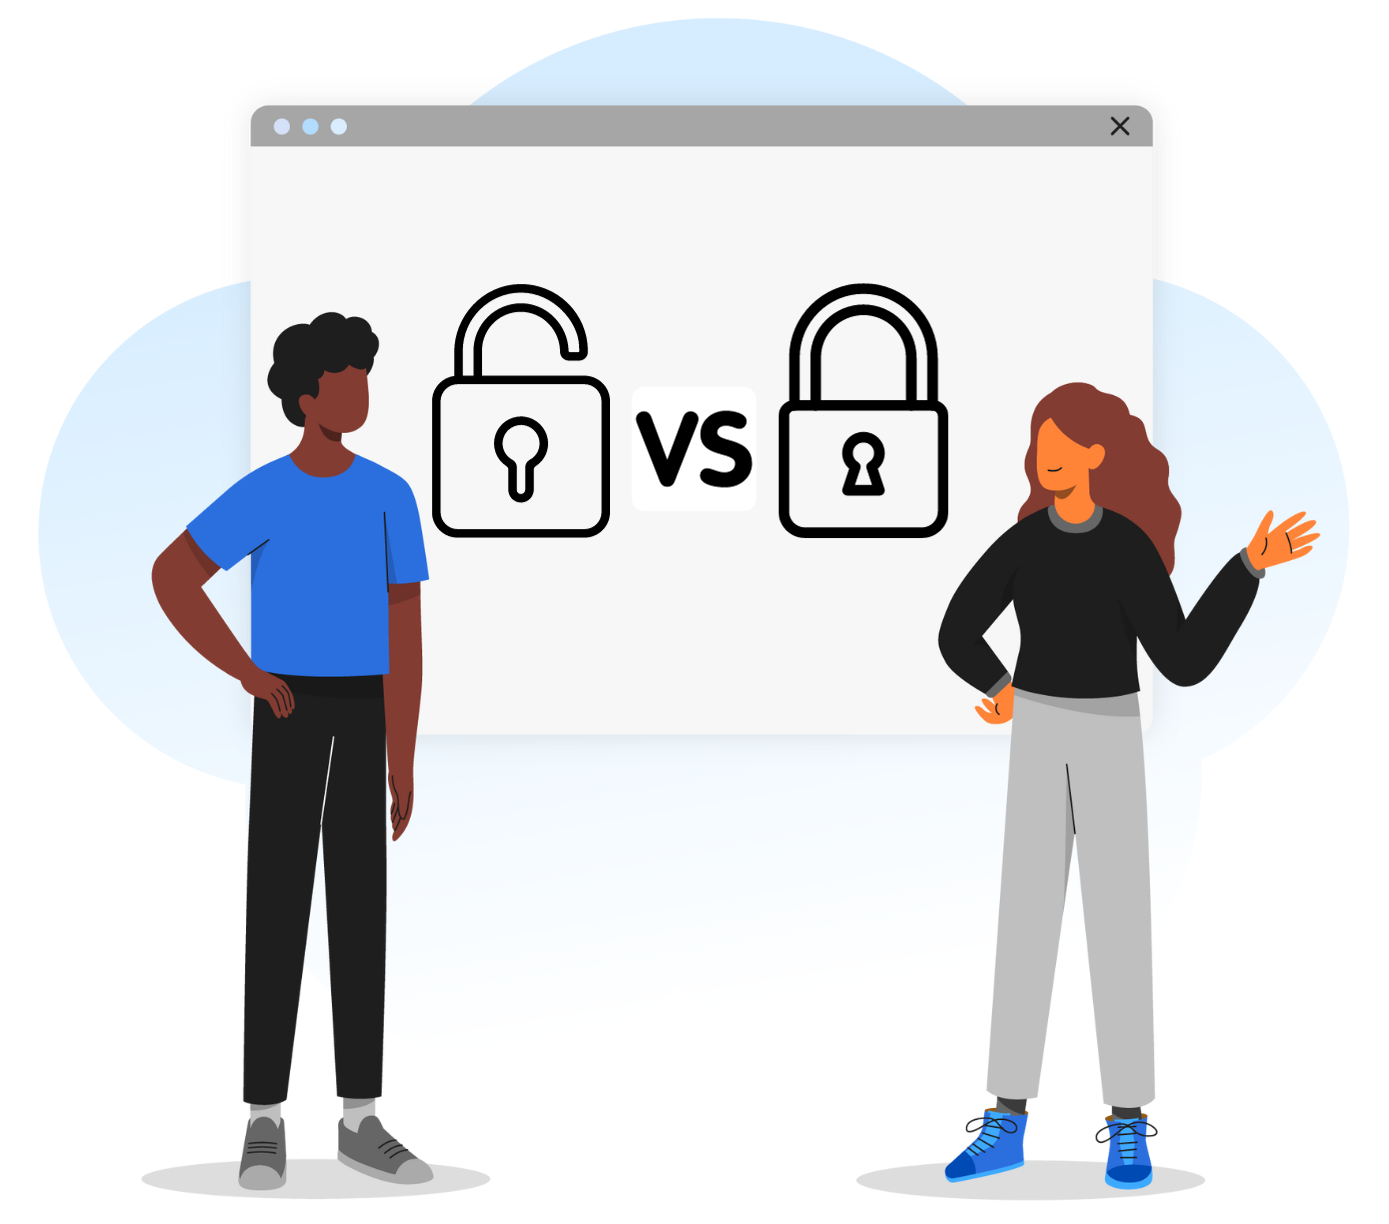
\includegraphics[scale=0.32]{Figures/0. General/open_vs_closed.png}
  \caption{\textit{Open source} contra \textit{Closed source}}
  \label{Open source vs. closed source}
\end{figure}